%!TEX root = TFG.tex

\chapter[Introduction]{Introduction}
%\addcontentsline{toc}{chapter}{Introduction}

% ----------------------------------------------------------

    The concept of Autonomous Vehicles introduces hopes for improvements to general locomotion, offering more security, comfort, and potential for new types of services. However, there are still obstacles which have to be worked on before its popularization: as the technology cultural/social acceptance and the required built-in cost.

    A possible solution to facilitate the dilution of the idea of machines driving general purpose vehicles would be to provide to users a visualization of what is being interpreted by the car algorithm. An approach that could also be implemented for case scenarios on supervision or surveillance. 

    The present work proposes the elaboration and development of a system for the representation in a 3D environment of the interpretation of autonomous cars algorithms as to provide a visualization interface for passengers.
    
    For the development and validation of the proposed system are used datasets with real-world images acquired by stereo cameras \cite{Geiger2013IJRR} and semantic images that distinguish different categories of objects in a scene such as cars, sidewalks, and vegetation \cite{giovaniThesis}. 
    
    Work was divided into the creation of two separate systems, the first one responsible for treating the input images and delivering as output a set of information for each identified entity in the scene, the second responsible for receiving entities and distributing them in an isolated graphical environment with predefined models in the correct position and size. The complete system data flow is shown in \autoref{fig:system-flowchart}.
        
    \begin{figure}[H]
         \caption{\label{fig:system-flowchart}System flowchart}
         \begin{center}
            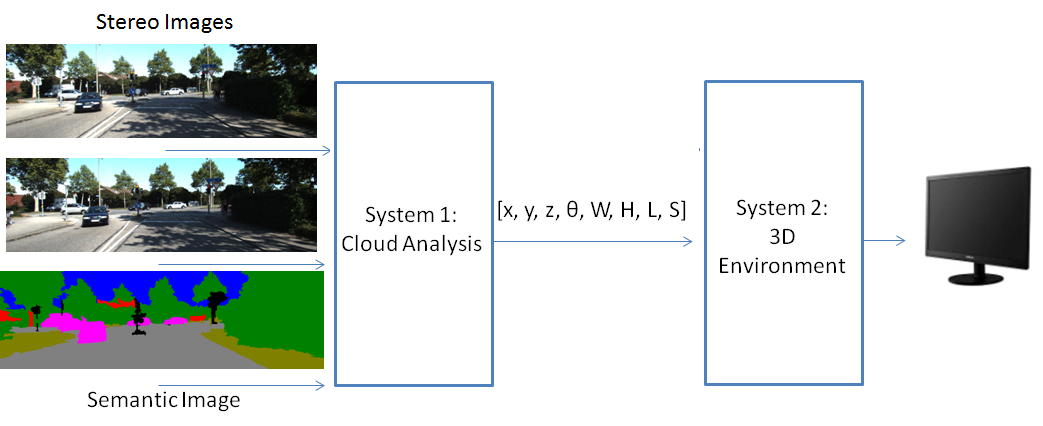
\includegraphics[width=0.85\textwidth]{images/proposed-system-flow-chart.png}
         \end{center}
         \legend{Source: Authors of this study.}
    \end{figure}
    
    The first system named Cloud Analysis is defined by four significant steps: disparity image generation, point cloud creation, semantic association, and feature extraction. It uses concepts of object-oriented programming \cite{object-oriented-modeling-and-design} in its implementation to organize data behavior.
    
    The second system is named 3D environment and has as input information of entities, it represents them in a 3D simulation using computer graphics. The concepts of Entity-Component Systems \cite{house-entity-component-explanation-stack} and Data-Oriented Design \cite{llopis-game-engine-gems-2} are used in its implementation as an approach for better performance results, thus requiring a more in-depth modeling of components and execution flow, which are explored in the development section.

    As contribution, this project delivers an approximation of the environment identified by computer vision algorithms. The system purpose is to bring more confidence to users by offering an interface dedicated to the understanding of algorithms running underneath autonomous vehicles. As future contribution the system can be used for data visualization in case scenarios of surveillance, or accidents by the processing of stored data. 

\section{General Objective}
    
    Elaboration and development of a software for embedded systems to create an estimated representation of the interpretations of Computer Vision algorithms for Autonomous Vehicles.
    
\section{Specific Objectives}

\begin{itemize}
    \item Creating 3D scenes with discriminating categories of objects from generated points clouds using disparity and semantic images;
    \item Describing entities in scenes using feature extraction;
    \item Survey of adequate software architectures and implementations for 3D Environment development;
    \item Development of the 3D Environment visualization software.
\end{itemize}
